\subsubsection{\stid{2.10} PROTEAS-TUNE: Autotuning} 

\paragraph{Overview}

We are developing tools and an application development workflow that separates a high-level C/C++/FORTRAN implementation from an architecture-specific implementation (OpenMP, CUDA, etc.), optimization, and  tuning.   This  approach
will enable Exascale application  developers to express and  maintain a
single, portable implementation of their computation that is also legal code
that can be compiled and run by using standard tools.   The autotuning compiler
and search framework will transform the baseline code into a   collection of
highly-optimized implementations. This reduces the need for extensive manual tuning.
Both code transformation and autotuning are essential in ECP for providing
performance portability on Exascale platforms.  Due to significant architectural
differences in ECP platforms, attaining performance portability may  require
fundamentally different  implementations of software -- different strategies for
parallelization, loop order,  data layout, and exploiting SIMD/SIMT.  A key
concern of ECP is the high cost of developing  and maintaining
performance-portable applications for  diverse Exascale architectures, including
manycore CPUs and GPUs. 
Ideally Exascale application developers would express their
computation separate from   its mapping to hardware, while autotuning compilers can automate this mapping and achieve performance portability.

\paragraph{Key  Challenges}
Autotuning has the potential to dramatically improve the performance portability of Petascale and Exascale applications.  To date, autotuning has been used primarily in high-performance applications through tunable libraries or previously tuned application code that is integrated directly into the application.
If autotuning is to be widely used in the HPC community,
support for autotuning must address the software engineering challenges, manage configuration overheads, and continue to demonstrate significant performance gains and portability across architectures.
In particular, tools that configure the application must be integrated into the application build process so that tuning can be reapplied as the application and target architectures evolve.

\paragraph{Solution Strategy}
We are developing pluggable software infrastructure that incorporates
autotuning at different levels: compiler optimization, runtime configuration of application-level parameters and system software.
To guarantee success in the ECP time frame, we are collaborating with
application teams, such as SuperLU and QMCPACK, to impact performance of their
codes and libraries.

The autotuning compiler strategy revolves CHiLL, which has the following distinguishing features:
(1) \textit{Composable transformation and code generation}, such
that the same tool can be applied
to multiple different application domains;
(2) \textit{Extensible to new domain-specific transformations} that can be represented as transformations on loop nest iteration spaces are also
composable with existing transformations;
(3) \textit{Optimization strategies and parameters exposed to autotuning:}
By exposing high-level expression
of the autotuning search space as transformation recipes, the compiler writer, an expert programmer or embedded DSL designer can directly \
express how to compose
 transformations that lead to different implementations.
A part of our efforts in ECP are to migrate these capabilities of CHiLL
into the Clang/LLVM open-source compiler, as well as provide lightweight
interfaces through Python, C++, and REST APIs/web services.

For example, we have developed a \textit{brick data layout library and code generator} for
stencil computations within CHiLL.
Recent trends in computer architecture that favor computation over data movement incentivize high-order methods.  Paradoxically, high-order codes can be challenging for compilers/optimization to attain high performance.  Bricks enable high performance and make fine-grained data reuse and memory access information known at compile time.  The SIMD code generation achieves performance portability
for high-order stencils for both CPUs with wide SIMD units (Intel Knights
Landing) and GPUs (NVIDIA Pascall).  Integration with autotuning attains
performance that is close to Roofline performance bound for both manycore CPU
and GPU architectures.

The Search using Random Forests (SuRF) search framework is a separate tool in Y-Tune that optimizes the search over an autotuning search space.  While
SuRF provides support to CHiLL for compiler-directed autotuning, it can
also be integrated directly with applications and runtimes to search over
application parameters and alternative code variants.
SuRF is an asynchronous search framework that consists of sampling a small number of input parameter configurations and progressively fitting a surrogate model over the input-output space until exhausting the user-defined maximum number of evaluations. The framework is designed to operate in the master-worker computational paradigm, where one master node fits the surrogate model and generates promising input configurations and worker nodes perform the computationally expensive evaluations and return the outputs to the master node. We implemented both MPI- and scheduler-based master-worker approaches.


\paragraph{Recent Progress}


We have pursued the following main activities this year:


\textit{ytopt Autotuning Framework:}
Previously we used our SuRF (Search using Random Forest) algorithm~\cite{nelson2015surf} as an ad-hoc implementation when used in our autotuning experiments. To support more reusability, we developed into into an autotuning framework support several additional machine learning methods. It is available at \url{https://github.com/ytopt-team/ytopt}. In contrast to other autotuning frameworks such as OpenTuner and ATF, it is more focused on our High Performance- and Scientific Computing use cases. 
ytopt samples a small number of input parameter configurations, evaluating them, and progressively fits a surrogate model over the input-output space until exhausting the user-defined time or maximum number of evaluations.
The framework provides two different class of methods: Bayesian Optimization and Reinforcement Learning. The software is designed to operate in the master-worker computational paradigm, where one master node fits the surrogate model and generates promising input configurations and worker nodes perform the computationally expensive evaluations and return the outputs to the master node. The asynchronous aspect of the search allows the search to avoid waiting for all the evaluation results before proceeding to the next iteration. As soon as an evaluation is finished, the data is used to retrain the surrogate model, which is then used to bias the search toward the promising configurations.


\textit{Autotuning Experiments:} 
We applied our algorithms and autotuning software to common scientific computing kernels. In the publication~\cite{sreenivasan2019openmp} we applied SuRF to autotuning parallelization parameters, such as scheduling algorithms and granularity. It makes use of a new component to apply directives to source code called Plopper.
We also combined Plopper with ytopt with our user-directed loop transformations~\cite{wu2020autotuning}. Thanks to ytopt, this allows using more machine algorithms, including SuRF. The additional user-directives~\cite{kruse2018pragmas} also enable more opportunities than just parallelization, such as loop interchange, tiling and array packing (extracting local working set to optimize for a cache level).


\textit{Tree-Shaped Search Space:}
The search space used by most machine learning methods is different from the structure of loop transformation composition. Loop transformations are best represented as a tree, as shown in Figure~\ref{fig:YTune-mctree}. This mismatch necessarily results in either optimization possibilities not being able to be found by the autotuner because they cannot be represented, and/or search inefficiencies because the relationships between optimization opportunities is not well-represented.
Therefore we developed an autotuner that is based on a tree-shaped search space~\cite{kruse2020search}. It can represent any composition of loop transformations. From the beginning we intend to use Monte-Carlo tree search as the machine learning algorithm, but have not implemented it yet. The current, simpler search strategy is promising, but tends to find local optima.

\begin{figure}[h]                                                                                               
\begin{center}
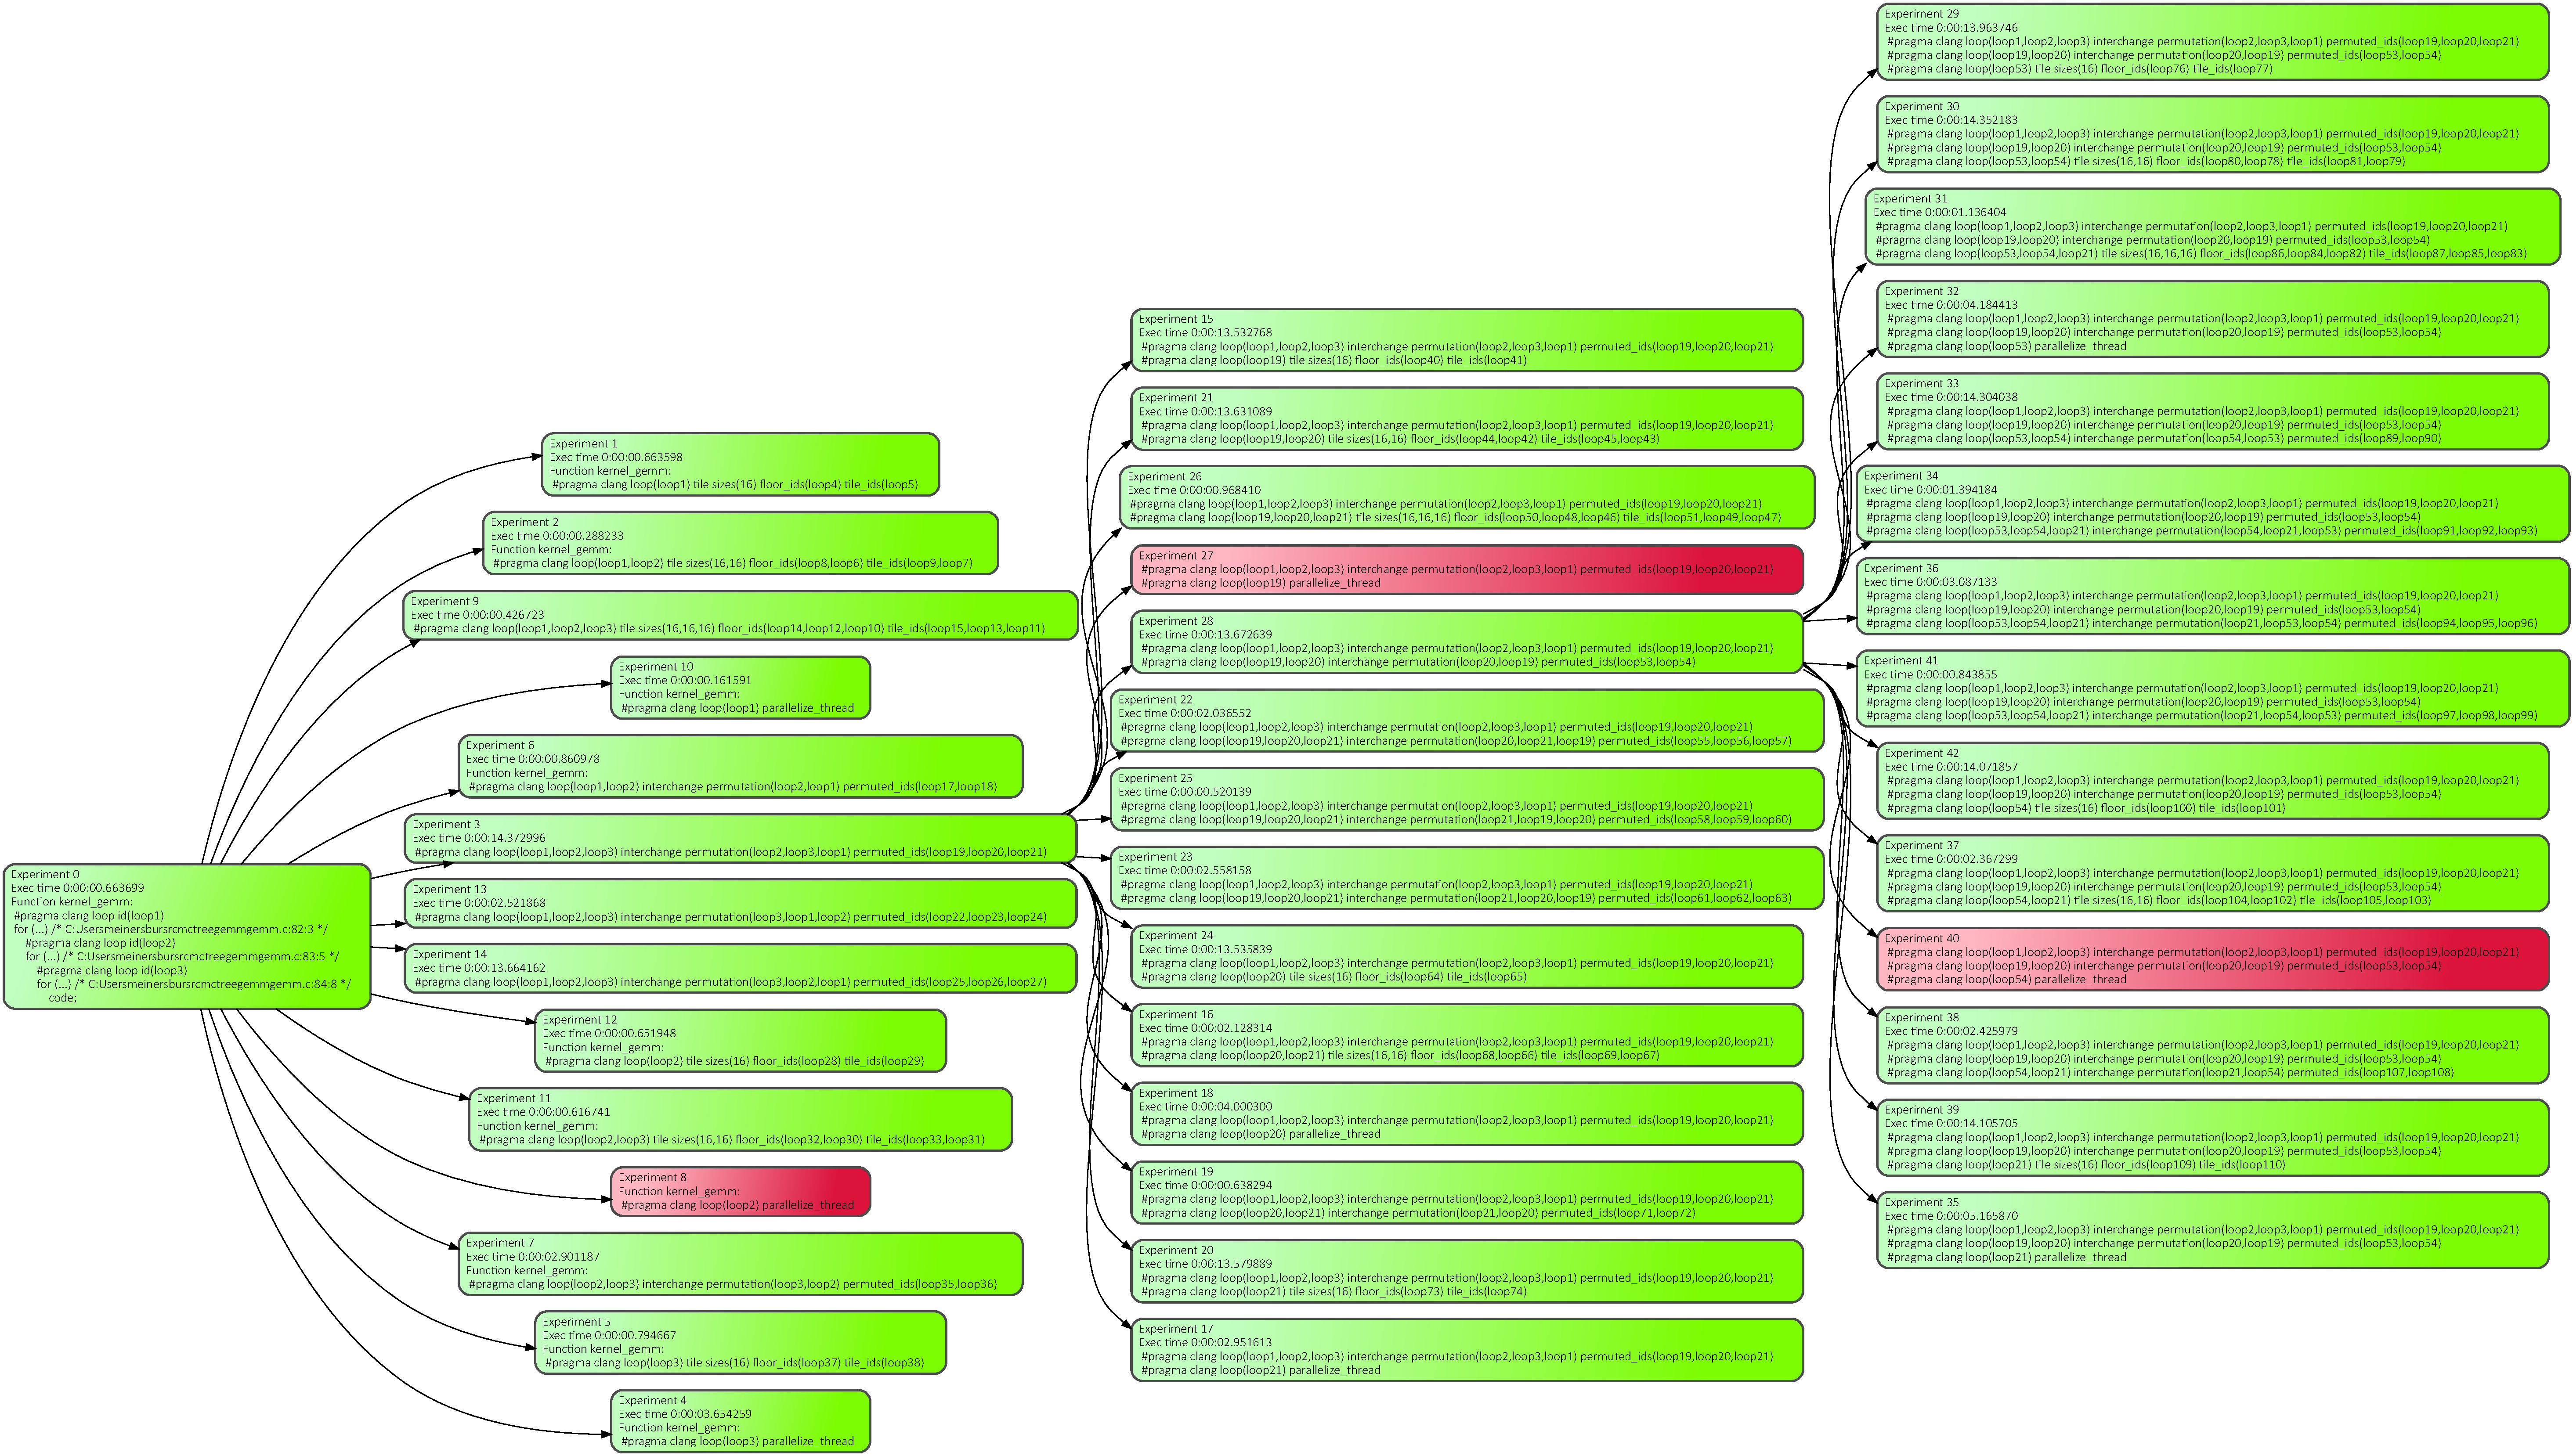
\includegraphics[width=0.7\textwidth]{projects/2.3.2-Tools/2.3.2.10-PROTEAS-YTUNE/YTune-searchtree}
\end{center}
\caption{Loop Optimization Search Space.}\label{fig:YTune-mctree}                                                                                    
\end{figure}


\paragraph{Next Steps}

We will continue to use apply our autotuning solution to more problems, including larger kernels from ECP applications. 
As mentioned, we are working on a new tree-shaped search space for autotuning which we are going to improve further. In particular, we are goinf to implement Monte-Carlo tree search (MCTS) to replace the current prototype algorithm. MCTS is a standard algorithm for trees and has been applied successfully to e.g. Chess. Moreover, we want to support more loop optimizations such as index-set splitting.
